
%% bare_adv.tex
%% V1.4b
%% 2015/08/26
%% by Michael Shell
%% See: 
%% http://www.michaelshell.org/
%% for current contact information.
%%
%% This is a skeleton file demonstrating the advanced use of IEEEtran.cls
%% (requires IEEEtran.cls version 1.8b or later) with an IEEE Computer
%% Society journal paper.
%%
%% Support sites:
%% http://www.michaelshell.org/tex/ieeetran/
%% http://www.ctan.org/pkg/ieeetran
%% and
%% http://www.ieee.org/

%%*************************************************************************
%% Legal Notice:
%% This code is offered as-is without any warranty either expressed or
%% implied; without even the implied warranty of MERCHANTABILITY or
%% FITNESS FOR A PARTICULAR PURPOSE! 
%% User assumes all risk.
%% In no event shall the IEEE or any contributor to this code be liable for
%% any damages or losses, including, but not limited to, incidental,
%% consequential, or any other damages, resulting from the use or misuse
%% of any information contained here.
%%
%% All comments are the opinions of their respective authors and are not
%% necessarily endorsed by the IEEE.
%%
%% This work is distributed under the LaTeX Project Public License (LPPL)
%% ( http://www.latex-project.org/ ) version 1.3, and may be freely used,
%% distributed and modified. A copy of the LPPL, version 1.3, is included
%% in the base LaTeX documentation of all distributions of LaTeX released
%% 2003/12/01 or later.
%% Retain all contribution notices and credits.
%% ** Modified files should be clearly indicated as such, including  **
%% ** renaming them and changing author support contact information. **
%%*************************************************************************


% *** Authors should verify (and, if needed, correct) their LaTeX system  ***
% *** with the testflow diagnostic prior to trusting their LaTeX platform ***
% *** with production work. The IEEE's font choices and paper sizes can   ***
% *** trigger bugs that do not appear when using other class files.       ***
% The testflow support page is at:
% http://www.michaelshell.org/tex/testflow/






\documentclass[10pt,journal,compsoc]{IEEEtran}

% *** CITATION PACKAGES ***
%
% \ifCLASSOPTIONcompsoc
%   % The IEEE Computer Society needs nocompress option
%   % requires cite.sty v4.0 or later (November 2003)
%   \usepackage[nocompress]{cite}
% \else
%   % normal IEEE
%   \usepackage{cite}
% \fi
% cite.sty was written by Donald Arseneau
% V1.6 and later of IEEEtran pre-defines the format of the cite.sty package
% \cite{} output to follow that of the IEEE. Loading the cite package will
% result in citation numbers being automatically sorted and properly
% "compressed/ranged". e.g., [1], [9], [2], [7], [5], [6] without using
% cite.sty will become [1], [2], [5]--[7], [9] using cite.sty. cite.sty's
% \cite will automatically add leading space, if needed. Use cite.sty's
% noadjust option (cite.sty V3.8 and later) if you want to turn this off
% such as if a citation ever needs to be enclosed in parenthesis.
% cite.sty is already installed on most LaTeX systems. Be sure and use
% version 5.0 (2009-03-20) and later if using hyperref.sty.
% The latest version can be obtained at:
% http://www.ctan.org/pkg/cite
% The documentation is contained in the cite.sty file itself.
%
% Note that some packages require special options to format as the Computer
% Society requires. In particular, Computer Society  papers do not use
% compressed citation ranges as is done in typical IEEE papers
% (e.g., [1]-[4]). Instead, they list every citation separately in order
% (e.g., [1], [2], [3], [4]). To get the latter we need to load the cite
% package with the nocompress option which is supported by cite.sty v4.0
% and later.


\usepackage{enumitem} 



% *** GRAPHICS RELATED PACKAGES ***
%
\ifCLASSINFOpdf
   \usepackage[pdftex]{graphicx}
  % declare the path(s) where your graphic files are
   \graphicspath{{./resources/}}
  % \graphicspath{{../pdf/}{../jpeg/}}
  % and their extensions so you won't have to specify these with
  % every instance of \includegraphics
   \DeclareGraphicsExtensions{.pdf,.jpeg,.png}
\else
  % or other class option (dvipsone, dvipdf, if not using dvips). graphicx
  % will default to the driver specified in the system graphics.cfg if no
  % driver is specified.
  % \usepackage[dvips]{graphicx}
  % declare the path(s) where your graphic files are
  % \graphicspath{{../eps/}}
  % and their extensions so you won't have to specify these with
  % every instance of \includegraphics
  % \DeclareGraphicsExtensions{.eps}
\fi
% graphicx was written by David Carlisle and Sebastian Rahtz. It is
% required if you want graphics, photos, etc. graphicx.sty is already
% installed on most LaTeX systems. The latest version and documentation
% can be obtained at: 
% http://www.ctan.org/pkg/graphicx
% Another good source of documentation is "Using Imported Graphics in
% LaTeX2e" by Keith Reckdahl which can be found at:
% http://www.ctan.org/pkg/epslatex
%
% latex, and pdflatex in dvi mode, support graphics in encapsulated
% postscript (.eps) format. pdflatex in pdf mode supports graphics
% in .pdf, .jpeg, .png and .mps (metapost) formats. Users should ensure
% that all non-photo figures use a vector format (.eps, .pdf, .mps) and
% not a bitmapped formats (.jpeg, .png). The IEEE frowns on bitmapped formats
% which can result in "jaggedy"/blurry rendering of lines and letters as
% well as large increases in file sizes.
%
% You can find documentation about the pdfTeX application at:
% http://www.tug.org/applications/pdftex





% *** MATH PACKAGES ***
%
\usepackage{amsmath}
% A popular package from the American Mathematical Society that provides
% many useful and powerful commands for dealing with mathematics.
%
% Note that the amsmath package sets \interdisplaylinepenalty to 10000
% thus preventing page breaks from occurring within multiline equations. Use:
\interdisplaylinepenalty=2500
% after loading amsmath to restore such page breaks as IEEEtran.cls normally
% does. amsmath.sty is already installed on most LaTeX systems. The latest
% version and documentation can be obtained at:
% http://www.ctan.org/pkg/amsmath





\usepackage{algorithm}
\usepackage{algorithmic}
% algorithmic.sty was written by Peter Williams and Rogerio Brito.
% This package provides an algorithmic environment for describing algorithms.
% You can use the algorithmic environment in-text or within a figure
% environment to provide for a floating algorithm. Do NOT use the algorithm
% floating environment provided by algorithm.sty (by the same authors) or
% algorithm2e.sty (by Christophe Fiorio) as the IEEE does not use dedicated
% algorithm float types and packages that provide these will not provide
% correct IEEE style captions. The latest version and documentation of
% algorithmic.sty can be obtained at:
% http://www.ctan.org/pkg/algorithms
% Also of interest may be the (relatively newer and more customizable)
% algorithmicx.sty package by Szasz Janos:
% http://www.ctan.org/pkg/algorithmicx








% *** PDF, URL AND HYPERLINK PACKAGES ***
%
%\usepackage{url}
% url.sty was written by Donald Arseneau. It provides better support for
% handling and breaking URLs. url.sty is already installed on most LaTeX
% systems. The latest version and documentation can be obtained at:
% http://www.ctan.org/pkg/url
% Basically, \url{my_url_here}.


% NOTE: PDF hyperlink and bookmark features are not required in IEEE
%       papers and their use requires extra complexity and work.
% *** IF USING HYPERREF BE SURE AND CHANGE THE EXAMPLE PDF ***
% *** TITLE/SUBJECT/AUTHOR/KEYWORDS INFO BELOW!!           ***
\newcommand\MYhyperrefoptions{
    bookmarks=true,
    bookmarksnumbered=true,
    pdfpagemode={UseOutlines},
    plainpages=false,
    pdfpagelabels=true,
    colorlinks=true,
    linkcolor={black},
    citecolor={black},
    urlcolor={black},
    pdftitle={A0209166A},%<!CHANGE!
% pdfsubject={Cryptography},%<!CHANGE!
    pdfauthor={SHEN Jiamin},%<!CHANGE!
% pdfkeywords={}
}%<^!CHANGE!
%\ifCLASSINFOpdf
%\usepackage[\MYhyperrefoptions,pdftex]{hyperref}
%\else
%\usepackage[\MYhyperrefoptions,breaklinks=true,dvips]{hyperref}
%\usepackage{breakurl}
%\fi
% One significant drawback of using hyperref under DVI output is that the
% LaTeX compiler cannot break URLs across lines or pages as can be done
% under pdfLaTeX's PDF output via the hyperref pdftex driver. This is
% probably the single most important capability distinction between the
% DVI and PDF output. Perhaps surprisingly, all the other PDF features
% (PDF bookmarks, thumbnails, etc.) can be preserved in
% .tex->.dvi->.ps->.pdf workflow if the respective packages/scripts are
% loaded/invoked with the correct driver options (dvips, etc.). 
% As most IEEE papers use URLs sparingly (mainly in the references), this
% may not be as big an issue as with other publications.
%
% That said, Vilar Camara Neto created his breakurl.sty package which
% permits hyperref to easily break URLs even in dvi mode.
% Note that breakurl, unlike most other packages, must be loaded
% AFTER hyperref. The latest version of breakurl and its documentation can
% be obtained at:
% http://www.ctan.org/pkg/breakurl
% breakurl.sty is not for use under pdflatex pdf mode.
%
% The advanced features offer by hyperref.sty are not required for IEEE
% submission, so users should weigh these features against the added
% complexity of use.
% The package options above demonstrate how to enable PDF bookmarks
% (a type of table of contents viewable in Acrobat Reader) as well as
% PDF document information (title, subject, author and keywords) that is
% viewable in Acrobat reader's Document_Properties menu. PDF document
% information is also used extensively to automate the cataloging of PDF
% documents. The above set of options ensures that hyperlinks will not be
% colored in the text and thus will not be visible in the printed page,
% but will be active on "mouse over". USING COLORS OR OTHER HIGHLIGHTING
% OF HYPERLINKS CAN RESULT IN DOCUMENT REJECTION BY THE IEEE, especially if
% these appear on the "printed" page. IF IN DOUBT, ASK THE RELEVANT
% SUBMISSION EDITOR. You may need to add the option hypertexnames=false if
% you used duplicate equation numbers, etc., but this should not be needed
% in normal IEEE work.
% The latest version of hyperref and its documentation can be obtained at:
% http://www.ctan.org/pkg/hyperref



\usepackage{minted}
% *** Do not adjust lengths that control margins, column widths, etc. ***
% *** Do not use packages that alter fonts (such as pslatex).         ***
% There should be no need to do such things with IEEEtran.cls V1.6 and later.
% (Unless specifically asked to do so by the journal or conference you plan
% to submit to, of course. )

% correct bad hyphenation here
\hyphenation{op-tical net-works semi-conduc-tor}


\begin{document}

%
% paper title
% Titles are generally capitalized except for words such as a, an, and, as,
% at, but, by, for, in, nor, of, on, or, the, to and up, which are usually
% not capitalized unless they are the first or last word of the title.
% Linebreaks \\ can be used within to get better formatting as desired.
% Do not put math or special symbols in the title.
\title{Assignment 2 - PART I}

\author{SHEN~Jiamin 
    \thanks{\textbf{SHEN Jiamin}} 
    \thanks{Student ID: A0209166A} 
    \thanks{NUSNET ID: E0446373} 
    \thanks{\texttt{shen\_jiamin@comp.nus.edu.sg}}
}

% The paper headers
\markboth{CS4236 - Cryptography Theory and Practice}{SHEN Jiamin - A0209166A}

% make the title area
\maketitle

\section{Secret Key Encryption}

%%%%%%%%%%%%%%%%%%%%%%%%%%%%%%%%%%%%%%%%%%%%%%%%%%%%%%%%%%%%%%%%%%%%%%%%%%%%%%%%
\subsection{Encryption using Different Ciphers and Modes}

OpenSSL supports some different ciphers in module \texttt{enc}.
It can be used as 
\begin{verbatim}
    $ openssl enc <cipher-type> <arguments>
\end{verbatim}
where supported \texttt{<cipher-type>} can be found in 
\begin{verbatim}
    $ openssl enc -ciphers
\end{verbatim}

Arguments have different functions. 
To encrypt or decrypt a message, a flag should be added to declare the direction.
\begin{verbatim}
    -e                  Encrypt
    -d                  Decrypt
\end{verbatim}
To perform encryption or decryption, key and IV (or a passphrase) are required. These are declared by 
\begin{verbatim}
    -k val              Passphrase
    -K val              Raw key, in hex
    -iv val             IV in hex
\end{verbatim}
To read input from or write output to a file, filenames should be declared by 
\begin{verbatim}
    -in infile          Input file
    -out outfile        Output file
\end{verbatim}
Apart from that, flag \texttt{-p} can be used to print the iv and key used in the encryption or decryption.

For this section, I tried 2 different block ciphers in 3 different modes and a stream cipher.
Commands used and the output is screenshot as Fig.\ref{fig:p1_1}:

\begin{figure}[tb!]
\centering
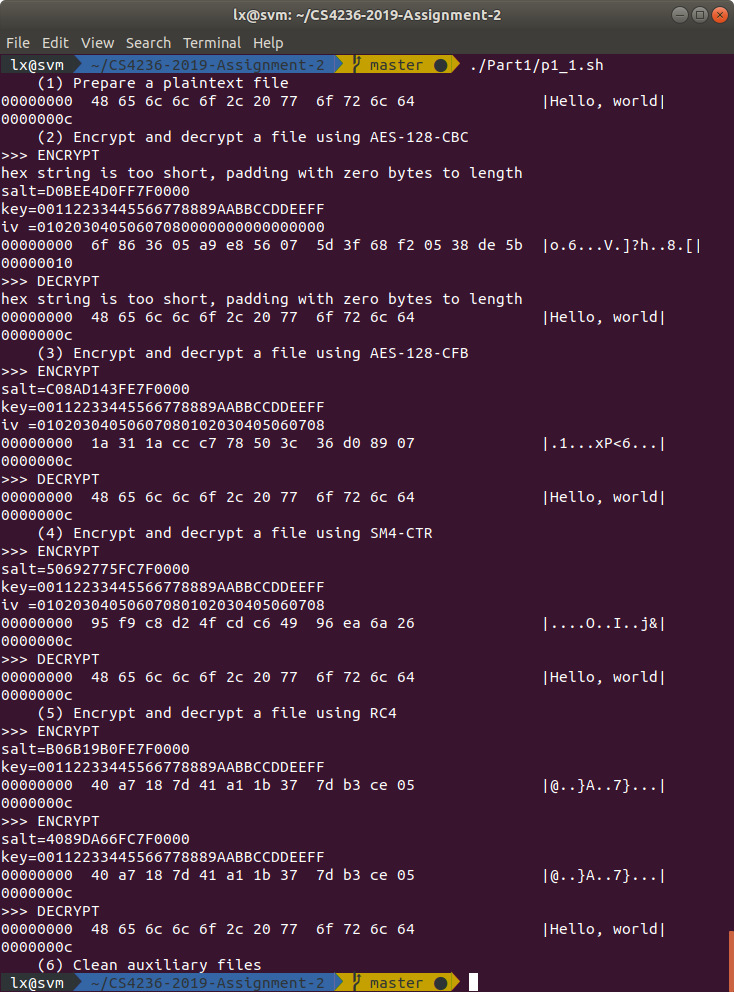
\includegraphics[width=\columnwidth]{pictures/p1_1.png}
\caption{
    Content in file \texttt{Part1/p1\_1.sh} is listed in Appendix \ref{code:1_1}
}
\label{fig:p1_1}
\end{figure}

\begin{enumerate}[label=(\arabic*)]
\item {
    \textbf{Output a string \texttt{Hello, world} into a file.} 
    The file will be encrypted later.
}
\item {
    \textbf{Encrypt and decrypt the file using AES block cipher in CBC mode with a key of 128 bits.} 
    In this part, I used the key and IV given.
    \begin{center}
        \texttt{Key = 00112233445566778889aabbccddeeff} \\
        \texttt{IV  = 0102030405060708}
    \end{center}
    Note that her IV has only 64 bits, but AES requires an IV of 128 bits. So there's a warning and the IV was padded with \texttt{0}. 
    Also Note that in CBC mode encryption, the length of ciphertext is an integer multiple of the block size. This is because, in CBC mode, the message was firstly padded and then encrypted.
}
\item {
    \textbf{Encrypt and decrypt the file using AES block cipher in CFB mode with a key of 128 bits. }
    In this part, I used the same key, but an IV of 128 bits to suppress the warning.
    \begin{center}
        \texttt{IV  = 01020304050607080102030405060708}
    \end{center}
    Note that in CFB mode, the length of ciphertext is the same as that of the message. This is because in CFB mode, a random stream is generated and XOR-ed with the message, so there's no need to pad the message.   
}
\item {
    \textbf{Encrypt and decrypt the file using SM4 block cipher in CTR mode.}
    SM4 only supports keys of 128 bits, so key length is not stated in the name of the cipher.
    In CTR mode, the length of ciphertext is also the same as that of the message.
}
\item {
    \textbf{Encrypt and decrypt the file using RC4 stream cipher with a key of 128 bits.}
    Note that IV is not required in RC4, so it should be a deterministic encryption scheme. Then I tried encrypting the same message twice using the same key, and two identical ciphertext was produced. Hence it is deterministic indeed.
    The length of ciphertext of RC4 is also the same as that of the message.
}
\end{enumerate}

%%%%%%%%%%%%%%%%%%%%%%%%%%%%%%%%%%%%%%%%%%%%%%%%%%%%%%%%%%%%%%%%%%%%%%%%%%%%%%%%
\subsection{Encryption Mode – ECB vs. CBC}

In this section, a picture is encrypted using AES in ECB mode and in CBC mode. The script used can be found in Appendix \ref{code:1_2}.

\begin{figure}[tb!]
\centering
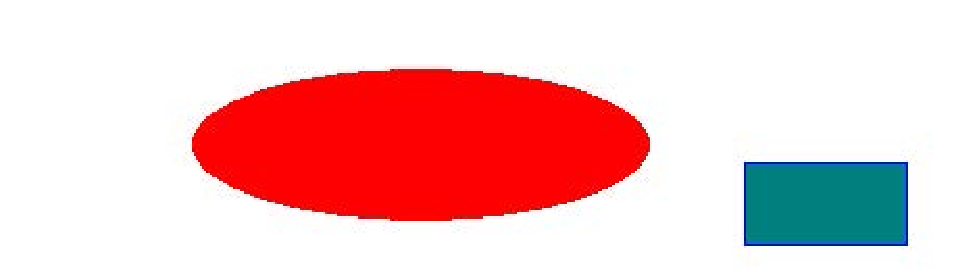
\includegraphics[width=\columnwidth]{pictures/pic_original.pdf}
\caption{
    The original picture
}
\label{fig:pic_original}
\end{figure}

\begin{figure}[tb!]
\centering
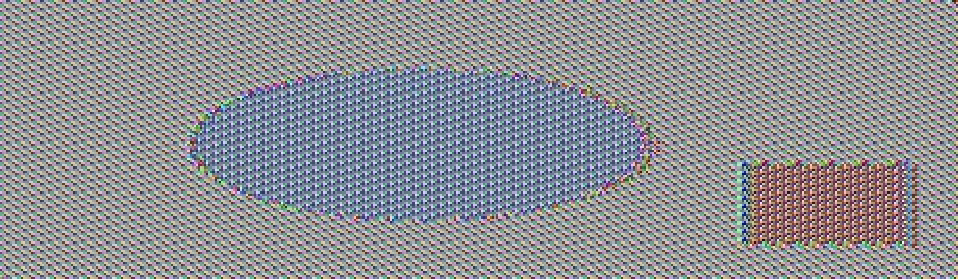
\includegraphics[width=\columnwidth]{pictures/pic_ecb.pdf}
\caption{
    The picture encrypted in ECB mode.
}
\label{fig:pic_ecb}
\end{figure}

\begin{figure}[tb!]
\centering

\includegraphics[width=\columnwidth]{pictures/pic_cbc.pdf}
\caption{
    The picture encrypted in CBC mode.
}
\label{fig:pic_cbc}
\end{figure}

\textbf{Observation.}
From the ECB-encrypted picture (Fig.\ref{fig:pic_ecb}), we can clearly see the edges of the graphics, which is the same as the original picture (Fig.\ref{fig:pic_original}).
While from the CBC-encrypted picture (Fig.\ref{fig:pic_cbc}), we can hardly find any information.

\begin{figure}[ht!]
\centering

\includegraphics[width=\columnwidth]{pictures/ECB_encryption.png}
\caption{
    Electronic Codebook (ECB) mode encryption \protect\footnotemark
}
\label{fig:ECB_encryption}
\end{figure}

\footnotetext{
    All the pictures showing mode of operation in this paper come from Wikipedia: \url{https://bit.ly/1CoRiM0}
}

\textbf{Explanation.}
In ECB mode (Fig.\ref{fig:ECB_encryption}), blocks of plaintext are encrypted using a block cipher under the same key. 
Then the blocks of ciphertext are concatenated to be the output.
Since the keyed block cipher is a deterministic function, the same blocks of plaintext was mapped to the same ciphertext.
Additionally, the diversity of blocks in the picture was really low.
Consequently, the colour information, which is based on a series of continuous bytes, was lost; while the shape information, which relies on the difference between several near blocks, was almost completely preserved. 

In CBC mode (Fig.\ref{fig:CBC_encryption}), each block of plaintext is firstly XOR-ed with the previous block of ciphertext. Therefore, although the keyed block cipher is deterministic, identical blocks are XOR-ed with different values and thus encoded as different ciphertext. So the shape information was also well hidden. 

The two examples also show that block cipher in CBC mode has a better property of diffusion than that in ECB mode.

\begin{figure}[ht!]
\centering

\includegraphics[width=\columnwidth]{pictures/CBC_encryption.png}
\caption{
    Cipher Block Chaining (CBC) mode encryption
}
\label{fig:CBC_encryption}
\end{figure}

%%%%%%%%%%%%%%%%%%%%%%%%%%%%%%%%%%%%%%%%%%%%%%%%%%%%%%%%%%%%%%%%%%%%%%%%%%%%%%%%
\subsection{Initialization Vector (IV)}

\subsubsection{}

AES-128-CBC is used for this section. Screenshot of the commands and outputs is as Fig.\ref{fig:p1_3_1}.

\begin{figure}[tb!]
\centering
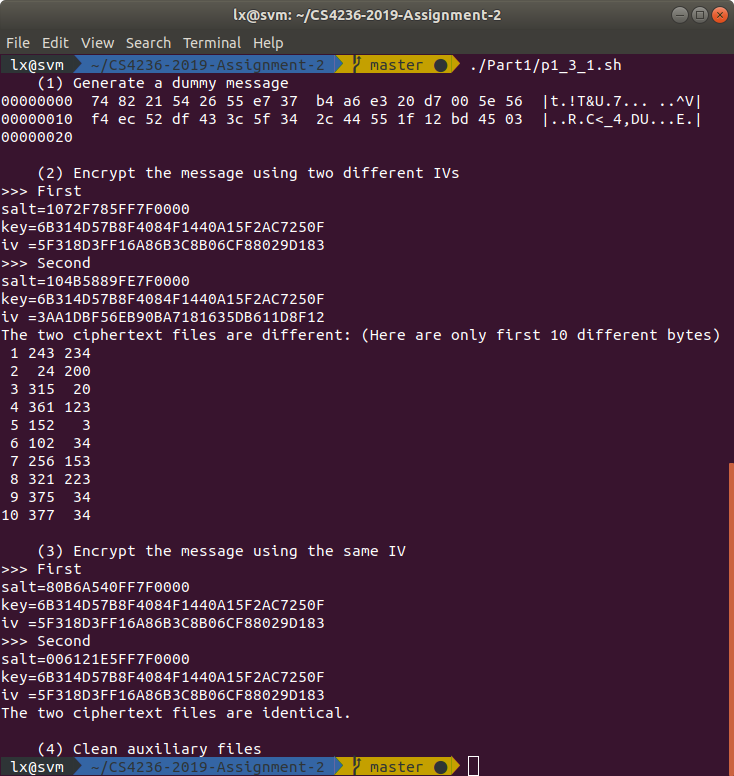
\includegraphics[width=\columnwidth]{pictures/p1_3_1.png}
\caption{
    Content in file \texttt{Part1/p1\_3\_1.sh} is listed in Appendix \ref{code:1_3_1}
}
\label{fig:p1_3_1}
\end{figure}

\textbf{Observation.}
From the outputs, it can be seen that when encrypting the same message under the same key, different ciphertext are produced with different IVs, while reusing IV leads to the same ciphertext.

\textbf{Explanation.}
CPA-security requires that the encryption scheme must be probabilistic. 
A probabilistic function has to be able to get access to a randomness source.

In the block cipher working in most modes of operation, IV (or counter in CTR mode) is the only source of randomness.
Hence if we reuse the IV (or even the IV can be predicated in CBC mode), the probabilistic function falls back to a deterministic function in the $\mathsf{PrivK}^{\mathsf{cpa}}$ game.

Therefore, in order to keep the encryption scheme producing different ciphertext for the same plaintext, IV can never be reused.

\subsubsection{}

\begin{figure}[tb!]
\centering
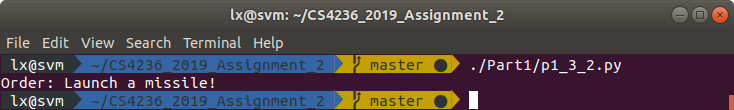
\includegraphics[width=\columnwidth]{pictures/p1_3_2.png}
\caption{
    Content in file \texttt{Part1/p1\_3\_2.sh} is listed in Appendix \ref{code:1_3_2}
}
\label{fig:p1_3_2}
\end{figure}

\textbf{In OFB mode.}
Yes, he/she can decrypt other messages that are not longer than the known message (\texttt{P1} in this problem). Screenshot of the commands and outputs is as Fig.\ref{fig:p1_3_2}.

\begin{figure}[ht!]
\centering

\includegraphics[width=\columnwidth]{pictures/OFB_encryption.png}
\caption{
    Output Feedback (OFB) mode encryption
}
\label{fig:OFB_encryption}
\end{figure}

OFB mode (Fig.\ref{fig:OFB_encryption}) generates a random stream from IV, and XOR-s the plaintext with the random stream generated. 
This can be stated as $$ c := G(IV) \oplus m $$ where pseudorandom generator $G$ is defined as $$
G_\infty(IV) := F_k(IV) || F_k(F_k(IV)) || \ldots
$$

Note that $G$ is a deterministic function. Thus when $G$ gets two inputs that are the same, it will produce two identical pseudorandom streams. That's to say $G(IV)$ becomes a constant value.

Since we already have a pair of plaintext $P_1$ and ciphertext $C_1$, we can calculate the first $|P_1|$ bytes of the random stream $R$ as $$
    R := P_1 \oplus C_1
$$ where $|R| = |P_1| = |C_1|$. Hence we can decrypt any ciphertext $C'$ where $|C'| \leq |R|$ by XOR-ing $C'$ with the first $|C'|$ bytes of $R$.

In this problem, $|C_1| = |C_2|$. So we can calculate $$
    P_2 = R \oplus C_2 = P_1 \oplus C_1 \oplus C_2
$$ directly.

\textbf{In CFB mode.}
If we use CFB mode (Fig.\ref{fig:CFB_encryption}) instead of OFB mode, we can only get the first block of a new message.

\begin{figure}[ht]
\centering

\includegraphics[width=\columnwidth]{pictures/CFB_encryption.png}
\caption{
    Cipher Feedback (CFB) mode encryption
}
\label{fig:CFB_encryption}
\end{figure}

While in OFB mode, the random stream is generated not only from the IV, but also influenced by the previous block of message. 
Hence although the IV and the key are the same, it can generate different random stream from different messages.

But we can still get the first block of message because $m_0 \oplus c_0$ always equals to $F_k(IV)$ where $m_0$ and $c_0$ are the first block of plaintext and ciphertext respectively. 
Thus adversary can calculate $F_k(IV)$ from any pair of plaintext and ciphertext, and then XOR the $F_k(IV)$ with the first block of ciphertext to reveal the first block of message.
This is sufficient to distinguish different messages and win the CPA game.

\subsubsection{}

Screenshot of the commands and outputs is as Fig.\ref{fig:p1_3_3}.

\begin{figure}[tb!]
\centering
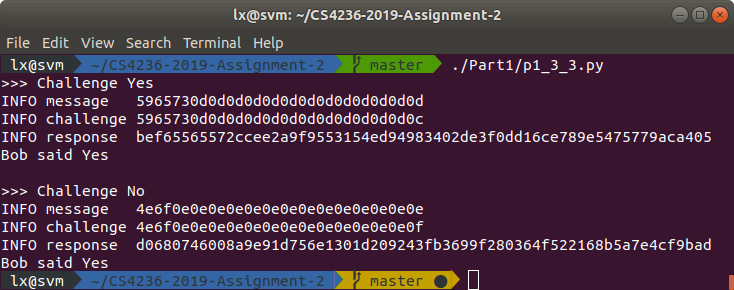
\includegraphics[width=\columnwidth]{pictures/p1_3_3.png}
\caption{
    Content in file \texttt{Part1/p1\_3\_3.sh} is listed in Appendix \ref{code:1_3_3}
}
\label{fig:p1_3_3}
\end{figure}

Note that the two messages are both shorter than a block, so it has to be padded firstly. Let $m$ be the padded message, i.e. $|m|$ is equal to block size.

In CBC mode (Fig.\ref{fig:CBC_encryption}), the first block of ciphertext $$ C_1 := F_k(IV \oplus m) $$
Hence to solve this problem, we can keep $IV_1 \oplus m = IV_2 \oplus P_2$, where $m$ is padded \texttt{Yes} or \texttt{No} and $IV_1$ and $IV_2$ are known value. (I choose $m$ = \texttt{Yes} for description here. In the code, I did both.) Thus $$ P_2 := m \oplus IV_1 \oplus IV_2 $$ can be easily constructed. 

Then we ask Bob to encrypt the $P_2$. From the description above, it is clear that $|P_2|$ is equal to the block size. Thus Bob will add another padding block after $P_2$ and return a ciphertext $C_2$ of two blocks.
Finally, check if the first block of the ciphertext $C_2$ equals to the ciphertext $C_1$ we already known. If $C = C_1$, Bob sent \texttt{Yes} just now. Otherwise it should be \texttt{No}.


\section{Public Key Encryption}

Note: all codes in this section include a common header file, \texttt{Part1/p2\_common.h}, which can be found in Appendix \ref{code:2_common}.

%%%%%%%%%%%%%%%%%%%%%%%%%%%%%%%%%%%%%%%%%%%%%%%%%%%%%%%%%%%%%%%%%%%%%%%%%%%%%%%%
% \subsection{Background}
\setcounter{subsection}{1}

%%%%%%%%%%%%%%%%%%%%%%%%%%%%%%%%%%%%%%%%%%%%%%%%%%%%%%%%%%%%%%%%%%%%%%%%%%%%%%%%
\subsection{BIGNUM APIs}

For the following sections, I used these API.\footnote{This part of introduction referred to OpenSSL online documents: \url{https://www.openssl.org/docs/man1.1.1/man3}}

Function \texttt{BN\_new} is used to allocate and initialize a new \texttt{BIGNUM}.
Function \texttt{BN\_free} is used to free the components of the \texttt{BIGNUM}, and if it was created by \texttt{BN\_new()}, also the structure itself.
Function \texttt{BN\_dup} creates a new \texttt{BIGNUM} containing the value \texttt{from}.
\begin{verbatim}
  BIGNUM *BN_new(void);
  void BN_free(BIGNUM *a);
  BIGNUM *BN_dup(const BIGNUM *from);
\end{verbatim}

Function \texttt{BN\_bn2hex} is used to serialize a \texttt{BIGNUM} into a hex string.
Function \texttt{BN\_hex2bn} is used to deserialize a hex string into a \texttt{BIGNUM}.
\begin{verbatim}
  char *BN_bn2hex(const BIGNUM *a);
  int BN_hex2bn(BIGNUM **a, 
                const char *str);
\end{verbatim}

Function \texttt{BN\_sub\_word} subtracts a \texttt{BIGNUM} by \texttt{w}.
Function \texttt{BN\_mul} multiplies two \texttt{BIGNUM}s.
Function \texttt{BN\_mod\_inverse} calculates $a^{-1} \mod{n}$ and return a pointer to the result.
These three functions are used when calculating the private exponent $d$.

Function \texttt{BN\_mod\_exp} calculates modulus exponent. It is used when encrypting, decypting, signing and verifying.
\begin{verbatim}
  int BN_sub_word(BIGNUM *a, BN_ULONG w);
  int BN_mul(BIGNUM *r, BIGNUM *a, 
             BIGNUM *b, BN_CTX *ctx);
  BIGNUM *BN_mod_inverse(BIGNUM *r, 
                         BIGNUM *a, 
                         const BIGNUM *n,
                         BN_CTX *ctx);
  int BN_mod_exp(BIGNUM *r, BIGNUM *a, 
                 const BIGNUM *p,
                 const BIGNUM *m, 
                 BN_CTX *ctx);
\end{verbatim}

Some of the above functions requires a \texttt{BN\_CTX}, which is used to storage temporary \texttt{BIGNUM} and to cut down the overhead for allocating and releasing memory.
Function \texttt{BN\_CTX\_new} is used to allocate and initialize a \texttt{BN\_CTX} structure.
Function \texttt{BN\_CTX\_free} frees the components of the \texttt{BN\_CTX} and the structure itself.
\begin{verbatim}
  BN_CTX *BN_CTX_new(void);
  void BN_CTX_free(BN_CTX *c);
\end{verbatim}

For easier use of the functions, some helper functions are written in \texttt{p2\_common.h}, which can be found in Appendix \ref{code:2_common}.

%%%%%%%%%%%%%%%%%%%%%%%%%%%%%%%%%%%%%%%%%%%%%%%%%%%%%%%%%%%%%%%%%%%%%%%%%%%%%%%%
\subsection{Deriving the Private Key}

The algorithm to derive private exponent $d$ is stated as Algorithm \ref{alg:rsa_pqe_d}.
Command and output is screenshot as Fig.\ref{fig:p2_3}.
Code can be found in Appendix \ref{code:2_3}

\begin{figure}[b!]
\centering
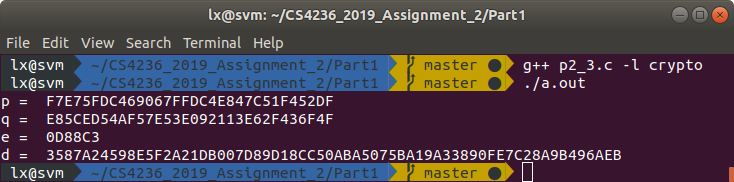
\includegraphics[width=\columnwidth]{pictures/p2_3.png}
\caption{
    Calculate private key exponent $d$
}
\label{fig:p2_3}
\end{figure}

\begin{algorithm}
\caption{Calculate private key exponent $d$}
\label{alg:rsa_pqe_d}
\begin{algorithmic}
\STATE \textbf{Input:} Private primes $p$,$q$ and public exponent $e$
\STATE \textbf{Output:} Private exponent $d$

\STATE $ n \gets pq $
\STATE $ \phi(n) \gets (p-1)(q-1) $
\STATE $ d \gets e^{-1} \mod{\phi(n)} $
\RETURN $ d $
\end{algorithmic}
\end{algorithm}

%%%%%%%%%%%%%%%%%%%%%%%%%%%%%%%%%%%%%%%%%%%%%%%%%%%%%%%%%%%%%%%%%%%%%%%%%%%%%%%%
\subsection{Encrypting a Message}

The algorithm to encrypt a message $m$ using RSA algorithm with public key $(n, e) $ is stated as Algorithm \ref{alg:rsa_enc}.
Command and output is screenshot as Fig.\ref{fig:p2_4}.
Code can be found in Appendix \ref{code:2_4}

\begin{algorithm}
\caption{RSA encrypt}
\label{alg:rsa_enc}
\begin{algorithmic}
\STATE \textbf{Input:} RSA public key $(n, e)$ and message $m$
\STATE \textbf{Output:} Ciphertext $c$

\STATE $ c \gets m^e \mod{n} $
\RETURN $ c $
\end{algorithmic}
\end{algorithm}

\begin{figure}[b!]
\centering
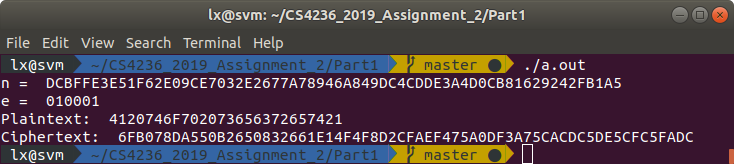
\includegraphics[width=\columnwidth]{pictures/p2_4.png}
\caption{
    RSA encrypt
}
\label{fig:p2_4}
\end{figure}

%%%%%%%%%%%%%%%%%%%%%%%%%%%%%%%%%%%%%%%%%%%%%%%%%%%%%%%%%%%%%%%%%%%%%%%%%%%%%%%%
\subsection{Decrypting a Message}

The algorithm to decrypt a ciphertext $c$ using RSA algorithm with private key $(n, d) $ is stated as Algorithm \ref{alg:rsa_dec}.
Command and output is screenshot as Fig.\ref{fig:p2_5}.
Code can be found in Appendix \ref{code:2_5}

\begin{algorithm}
\caption{RSA decrypt}
\label{alg:rsa_dec}
\begin{algorithmic}
\STATE \textbf{Input:} RSA private key $(n, d)$ and ciphertext $c$
\STATE \textbf{Output:} Plaintext $m$

\STATE $ m \gets c^d \mod{n} $
\RETURN $ m $
\end{algorithmic}
\end{algorithm}

\begin{figure}[b!]
\centering
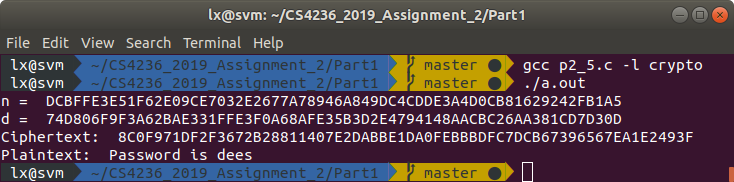
\includegraphics[width=\columnwidth]{pictures/p2_5.png}
\caption{
    RSA decrypt
}
\label{fig:p2_5}
\end{figure}

%%%%%%%%%%%%%%%%%%%%%%%%%%%%%%%%%%%%%%%%%%%%%%%%%%%%%%%%%%%%%%%%%%%%%%%%%%%%%%%%
\subsection{Signing a Message}
\label{subs:sign}

The algorithm to sign a message $m$ using RSA algorithm is completely the same as RSA decryption (Algorithm \ref{alg:rsa_dec}) which utilize the private key except that the output was called a signature.
Command and output is screenshot as Fig.\ref{fig:p2_6}.
Code can be found in Appendix \ref{code:2_6}

Note that when I changed \texttt{\$2000} to \texttt{\$3000}, the signature becomes different. Concretely, we changed 1 bit in the message. Then there are 123 different bits (in the total 256 bits) in the two signatures, which is nearly 50\% of all bits.

\begin{figure}[b!]
\centering
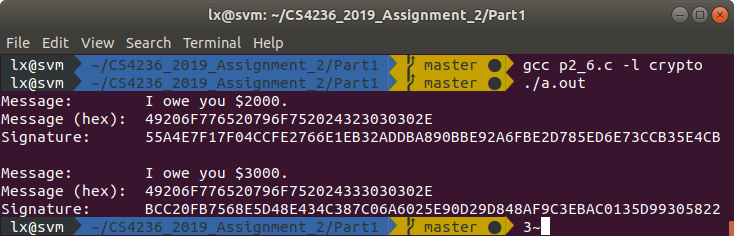
\includegraphics[width=\columnwidth]{pictures/p2_6.png}
\caption{
    RSA sign
}
\label{fig:p2_6}
\end{figure}

%%%%%%%%%%%%%%%%%%%%%%%%%%%%%%%%%%%%%%%%%%%%%%%%%%%%%%%%%%%%%%%%%%%%%%%%%%%%%%%%
\subsection{Verifying a Signature}

The algorithm to verify a signature using RSA algorithm is stated as Algorithm \ref{alg:rsa_verify}).
Command and output is screenshot as Fig.\ref{fig:p2_7}.
Code can be found in Appendix \ref{code:2_7}

From this example, it can be seen that 1 bit different in the two signature caused the recovered measurements completely different. They even don't have the same length.

This example and the one in Question \ref{subs:sign} show that there's a great diffusion property in RSA.

\begin{algorithm}
\caption{RSA verify}
\label{alg:rsa_verify}
\begin{algorithmic}
\STATE \textbf{Input:} RSA public key $(n, e)$, message $m$ and signature $S$
\STATE \textbf{Output:} \texttt{SUCCESS} or \texttt{FAIL}

\STATE $ s \gets m^e \mod{n} $

\IF {$S = s$} 
    \RETURN \texttt{SUCCESS}
\ELSE
    \RETURN \texttt{FAIL}
\ENDIF 

\end{algorithmic}
\end{algorithm}

\begin{figure}[b!]
\centering
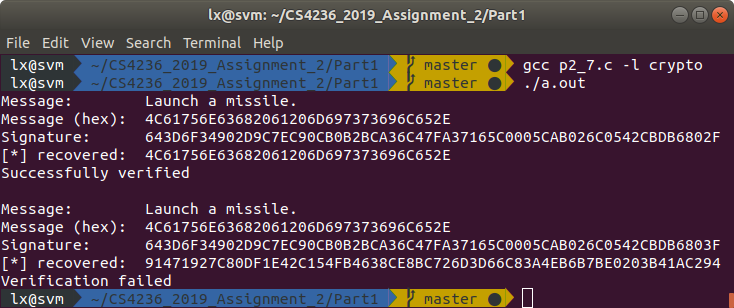
\includegraphics[width=\columnwidth]{pictures/p2_7.png}
\caption{
    RSA verify
}
\label{fig:p2_7}
\end{figure}

\newpage
\onecolumn

\appendices

\section{\texttt{Part1/p1\_1.sh}}
\label{code:1_1}
\inputminted{bash}{../Part1/p1_1.sh}
\newpage

\section{\texttt{Part1/p1\_2.sh}}
\label{code:1_2}
\inputminted{bash}{../Part1/p1_2.sh}
\newpage

\section{\texttt{Part1/p1\_3\_1.sh}}
\label{code:1_3_1}
\inputminted{bash}{../Part1/p1_3_1.sh}
\newpage

\section{\texttt{Part1/p1\_3\_2.py}}
\label{code:1_3_2}
\inputminted{python}{../Part1/p1_3_2.py}
\newpage

\section{\texttt{Part1/p1\_3\_3.py}}
\label{code:1_3_3}
\inputminted{python}{../Part1/p1_3_3.py}
\newpage

\section{\texttt{Part1/p2\_common.h}}
\label{code:2_common}
\inputminted{c}{../Part1/p2_common.h}
\newpage

\section{\texttt{Part1/p2\_3.c}}
\label{code:2_3}
\inputminted{c}{../Part1/p2_3.c}
\newpage

\section{\texttt{Part1/p2\_4.c}}
\label{code:2_4}
\inputminted{c}{../Part1/p2_4.c}
\newpage

\section{\texttt{Part1/p2\_5.c}}
\label{code:2_5}
\inputminted{c}{../Part1/p2_5.c}
\newpage

\section{\texttt{Part1/p2\_6.c}}
\label{code:2_6}
\inputminted{c}{../Part1/p2_6.c}
\newpage

\section{\texttt{Part1/p2\_7.c}}
\label{code:2_7}
\inputminted{c}{../Part1/p2_7.c}



\end{document}


